\subsection{Specifications and Requirements}
This project idea requires the integration of power, systems, computer, optical, and web engineering to achieve a final product of a self-sustaining plant bed. The design in \autoref{fig:overall-block} shows four different subsystems the team has designated as power, control, sensing, and web.
\begin{figure}[H]
    \caption{Overall block diagram}
    \centering
    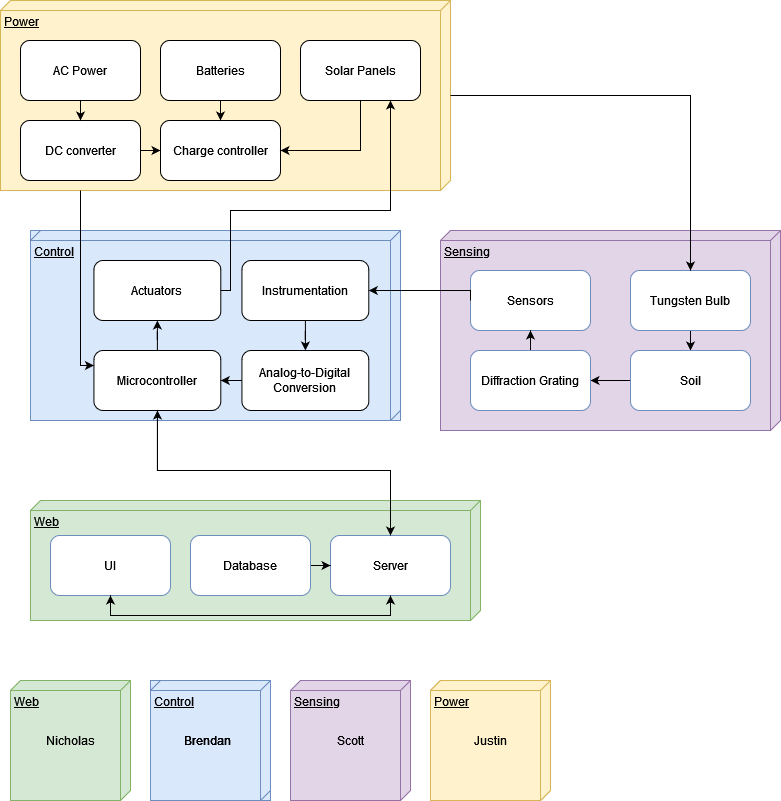
\includegraphics[width=\textwidth]{images/Overall Block Diagram.png}
    \label{fig:overall-block}
\end{figure}
\paragraph{Control}
The control subsystem is the brains of the entire operation. This subsystem has to accomplish four distinct tasks:
\begin{enumerate}
    \item Actuate mechanical components (linear rail, solenoid valve)
    \item Convert analog sensor data to digital data
    \item Send plant bed telemetry to web subsystem
    \item Receive commands from web subsystem and modify system accordingly
\end{enumerate}
In order to accomplish the first task, the chosen microcontroller (MCU) must be capable of driving the currents for these components and also support pulse-width modulation (PWM) for interacting with the motor controller. The second task requires that the MCU have an analog-to-digital converter. The third and fourth tasks necessitate WiFi connectivity as well as firmware support for either HTTP requests or WebSockets. These requirements for the control subsystem weigh heavily in the discussion of which MCU to choose found in Section \ref{sec:ps-control}.
\paragraph{Power}
The power system's function is self-explanatory, supply power to the entire system. This will be accomplished in two ways. First, using a DC barrel-plug to the wall, the system could be powered this way. The second way, is via the solar panels, batteries, and charge controller. Both manners of supplying power to the system must be regulated. Discussed in Section \ref{sec:ps-power} are the different ways that the charge controller can efficiently switch between battery power and the panels to increase battery health and charge level.
\paragraph{Sensing}
The sensing subsystem is where the majority of the novelty of this project lies. A lot of problems with electronic sensing is decay in the wet environs of plant beds. To improve upon this problem and hopefully offer a more sustainable and expandable approach, the team is going to try to accomplish sensing optically via infrared spectroscopy. Through the use of spectroscopy the team will be able to collect a wider range of data than just soil moisture content which includes soil OH group content, temperatue, and acidity.
\paragraph{Web}
The web component of this project accomplishes three things; data analysis, reporting, and user specified control of components. The data analysis is occurring on the web because of the greater availability of compute power and greater ease of programmability. For reporting, the web will use databases to store data ad infinitum and serve this data in the form of graphs or ``live'' metrics. The web component also will be able to take a user's input to send commands back to the control system to actuate different parts such as the solenoids or to ask for a more recent data reading.
\subsubsection{Engineering Specifications}
The team compiled a set of specifications for each of the subsystems that would need to be implemented to accomplish the requirements from above. \autoref{table:eng-specs} shows breaks down these specifications by the corresponding subystem.
\begin{table}[H]
    \caption{Engineering Specifications}
    \centering
    \begin{tabular}{c|c|c}
        \hline
        \textbf{Subsystem} & \textbf{Metric} & \textbf{Specification} \\\cline{2-3}
        \hline
        \multirow{8}{*}{\textbf{Control}} & Input voltage & 2.8-5.5 V \\ \cline{2-3}
                                        & Power consumption & $\leq$1.50W nominal power draw \\ \cline{2-3}
                                        & Shutdown power draw   & $\leq$100 uW \\ \cline{2-3}
                                        & Processor speed       & $\geq$20 MHz \\ \cline{2-3}
                                        & ADC resolution        & $\geq$8-bit \\ \cline{2-3}
                                        & ADC sampling rate     & $\geq$1 ksps \\ \cline{2-3}
                                        & Transmit power        & $\geq$10 dBm \\ \cline{2-3}
                                        & Receive sensitivity   & $\geq$-50 dBm \\ \cline{2-3}
        \hline
        \multirow{5}{*}{\textbf{Power}} & Power & 20-30W \\\cline{2-3}
                                        & Battery Capacity & 8Ah/95Wh \\\cline{2-3}
                                        & Battery Nominal Voltage & 9.6-12.8V \\\cline{2-3}
                                        & Charging Time & \textless4 hours \\\cline{2-3}
                                        & Regulator Efficiency & \textgreater65\% \\\cline{2-3}
        \hline
        \multirow{3}{*}{\textbf{Sensing}} & Spectra & 400nm - 1700nm \\\cline{2-3}
                                        & Resolution & \textless10nm \\\cline{2-3}
                                        & Output voltage range & 0-1.8V \\\cline{2-3}
        \hline
        \multirow{2}{*}{\textbf{Web}} & Up-time & 95\textpm.1\% \\\cline{2-3}
                                    & Storage Capacity & \textgreater16 GB \\\cline{2-3}
        \hline
        \multirow{2}{*}{\textbf{Miscellaneous}} & Dimensions & 1 m\textsuperscript{3} \\\cline{2-3}
                                                & Weight\tablefootnote{The weight of the system includes a full soil load} & \textless 50lb \\
        \hline
    \end{tabular}
    \label{table:eng-specs}
\end{table}
\paragraph{Control}
The specifications in the control portion of the table are focused on future integration. This is best exemplified by the need for a large ADC (above 8-bits) as well as the wireless capabilities. The power and voltage specifications are for convenience when integrating with the power subsystem.
\paragraph{Power}
The power specifications were made throughout the design process. For example, the power output was an unknown until all the subsystems had a firm idea of their power requirements. The maximum instantaneous power draw of the entire system is in the 20-30W range, hence where that specification is drawn from. The battery capacity and charging time are derived from the duration the team decided the system should last on battery power and the input power from the solar panels.
\paragraph{Sensing}
The spectra was chosen 
\paragraph{Web}
The web engineering specifications were hard to put into words. In general, the team wanted a reliable service quantified by the up-time of the web service. The service also needs to be able to store data in perpetuity for at least a single plantbed. Due to the efficiency of data storage and compression as well as the frequency of scans, the team felt that 16GB was effective enough to showcase the full system for now.
\paragraph{Miscellaneous}
The current miscellaneous specifications regard the physical qualities of the system. The dimensions of a meter cubed are necessary for the depth needed for various plants as well as solar panels. The weight is heavily correlated to weight of batteries, control and sensing components, as well as the soil and water hosing system. 
\subsubsection{Marketing Requirements}
When thinking about the target market for a project like this, the team put together a list of requirements important to the consumers. The most important feature for the consumer would be how easy the product is to use and navigate. This feature ranks the highest and would be the main determining factor on whether a consumer purchases this product over a competitor. Two other highly important features to a consumer would be the accuracy of the product and the cost. The accuracy is important because it directly correlates to the success of the customer's garden. If the product is not accurate in watering the plants, the customer will be unsatisfied and the plants will not survive. Cost because every consumer has to consider their budget - how much they are willing to spend for the features they deem most important. Other customer requirements the team brought up include the durability, configurability, environmental friendliness, portability and update frequency; listed from more important to less for consumer preferences. Each of these requirements have a direct correlation to at least one of the engineering requirements set for the product. \\

The engineering requirements set by the team are: weight of the product, dimensions of the product, battery life, how much power it consumes, up-time of the website, and quality of sensor resolution. \\

Many of the engineering requirements are directly correlated with each other. As weight improves, or lessens, so will product dimensions and vice versa. As dimensions decrease for the product, the amount of power needed decreases which means power consumption lessens which is also a positive correlation for the requirements. The only negative correlation in the engineering requirements the team found was that as sensor resolution increases, the life of the battery decreases as the lighting for the sensor must remain on longer. \\
 

\begin{figure}[H]
    \centering
    \caption{House of Quality}
    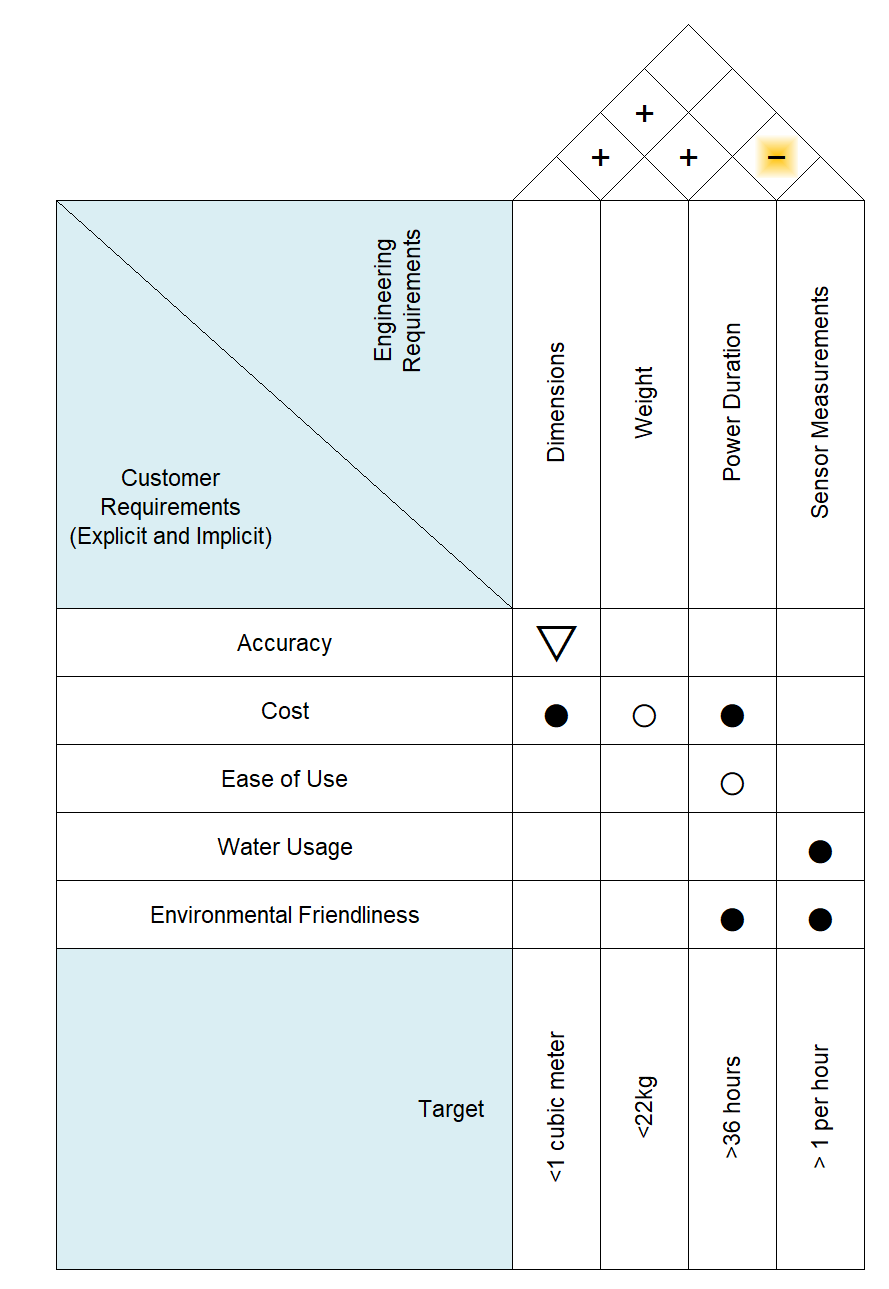
\includegraphics[width=\textwidth]{images/HouseOfQuality.PNG}
\end{figure}

When considering the customer requirement of ease of use, the team considered the impact of all the engineering requirements. Weight, battery life, and up-time all have a positive impact on customer experience. The lighter the product is, the easier it is for the customer to use because they can move it and adjust things within the product easier. The longer the batter life, the less time the consumer needs to worry when there are days with lower sunlight because the batteries can withstand a longer duration without being recharged. When the product has more up-time, the less time the consumer has to spend waiting on product updates. One of the engineering requirements that has a moderate impact on the customer experience is the sensor resolution. Although it can make a large impact on the overall product performance, its direct correlation to ease of use is not as strong as other requirements. The second most important marketing requirement listed by the team was accuracy. The only engineering requirement that had any correlation, had a strong correlation which is sensor resolution. This requirement is important to this marketing requirement because it could be a tipping point on whether a consumer purchases this product versus another. If the sensor resolution is not high enough to detect watering needs for the plant, the product will not be successful. This is why it is such an important requirement to focus on for both marketing and development of the product.\\

Something every team and every consumer is going to consider when designing or purchasing a product is the cost. The team rated this marketing requirement as an 8/10 for this product. It was not the highest priority because for a product like this, consumers will pay more to have a more accurate and easy-to-use product. The team also considered that customers using this product will do more research about the technical features because they are most likely growing fruits or vegetables that they will consume. Unfortunately, most things that increase the quality and appeal of the product, have a negative relationship that is strong in correlation. When the team looks at lighter materials, those materials increase the price. When adding a longer battery life and lowering power consumption, price will increase proportionally to how much those requirements change. To increase the resolution of the sensor, the team and consumers will have to pay more for the increase in quality and performace. The only requirement that  correlates to cost that was not strong, but still has an impact is the up-time. The more up-time of the product services, the more cost that is involved, but it is a smaller margin compared to the other requirements that directly impact the cost of the product. \\

Durability is most affected by the engineering requirements of weight and dimension. If the product materials are different, the durability will change and if the dimensions change shape or length, the construction will change affecting product strength. Weight will have a stronger impact on durability because it is something cosumers will consider more heavily and the materials will impact more. This is why weight has a strong correlation and dimensions are moderately correlated. Another marketing requirement that is similarly affected by weight and dimension is the portability of the product. The battery life also affects the portability. As battery life increases, so does the size and configuration of the battery which affects how easy it is to move. Weight has the largest affect on portability, followed by dimensions and then battery life. The configurability of the project is strongly affected by both dimension and power consumption. Battery life has a smaller affect on this, but still changes the set-up of the product. \\

Although environmental friendliness rates lower on the consideration for a consumer, it is affected by more engineering requirements. Battery life has a small impact on how environmentally friendly this product is because of the waste that will exist once the battery is retired. The factor considered most impactful is the power consumption. The greater the power consumption, the less friendly the product will be to the environment. If the team is able to focus on lowering the power consumption, marketing will be easiest for environmental friendliness. Up-time and sensor resolution have a moderate affect on this requirement and should have some connsideration in design of the product, but will be considered with more correlation to other requirements than environmental impact. \\

The last requirement comparison done by the team is update frequency. This marketing requirement is strongly correlated to up-time and moderately correlated to sensor resolution. Both of these engineering requirements affect the time spent on updating the software for the product. \\

\paragraph{Competition}
This product already has a competitive edge in the current market because it is unique. It will be the first all-inclusive garden bed that can be used outside. When looking at products that offer something similar, the team found two main options that a consumer may consider next to this product. The first competitor being considered is the Aero Garden. This product is a small indoor herb garden that provides UV light to help the plants thrive. A consumer wanting to start only an herb garden indoors may consider this product because it is more affordable, but would choose our product for its ease-of-use. The full garden bed design is more durable and waters the plants for the consumer. This is a big factor for a consumer to consider because many gardeners over or under water their plants. So although the Aero Garden may be more competitive indoors, the target market for our product will be won over with the requirements our team has focused on. The second competitor we considered is the FarmBot. This product is an automatic watering system that can be installed on an outside garden bed. When consumers glance at both of the products, they will automatically lean towards ours because of the value and price point. The FarmBot may have more accuracy, but not significant enough to justify the price difference. Additionally, this product is harder to assemble and larger which won't accomodate the average home-gardener. FarmBot is for a consumer that has more time, space, and money, but not for the majority of consumers.